\documentclass[12pt]{article}
\usepackage[a4paper]{geometry}
\usepackage{fullpage}
\usepackage[T1]{fontenc}
\usepackage[utf8]{inputenc}
\usepackage{graphicx}
\usepackage{mathpazo}
\pagenumbering{gobble}
\usepackage{siunitx}
\sisetup{output-decimal-marker = {,}}
\usepackage{amsmath}
\usepackage{esdiff}
\usepackage[spanish]{babel}
\usepackage{steinmetz}
\usepackage{pdfpages}

\begin{document}

\title{\textsc{Teoría de Circuitos II} \\ Convocatoria Extraordinaria}

\date{}

\maketitle

\section*{Equivalente de Thévenin}
Determina el generador equivalente de Thévenin del circuito de la figura entre los terminales A y B, y calcula la impedancia que hay que conectar entre estos terminales para conseguir que el circuito entregue la máxima potencia disponible, siguiendo estos pasos:

\begin{enumerate}
\item \textbf{(1p.)} Determina la tensión $U_{Z6}$ y la corriente $I_{Z2}$ para los generadores dependientes.
\item \textbf{(4p.)} Aplica movilidad a las fuentes de corriente para simplificar el circuito.
\item \textbf{(4p.)} En el circuito obtenido en el apartado anterior, aplica dominancia de fuentes, y nuevamente movilidad si fuese necesario.
\item \textbf{(1p.)} Con el circuito obtenido determina el generador equivalente de Thévenin, y calcula la impedancia que se debe conectar entre A y B.
\end{enumerate}

\begin{minipage}[c]{0.5\linewidth}
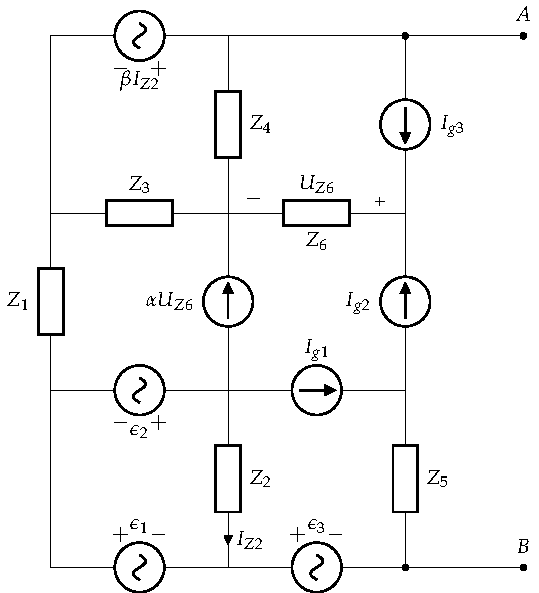
\includegraphics[]{figs/thevenin.pdf}  
\end{minipage}
\begin{minipage}[c]{0.5\linewidth}
  \begin{align*}
    \overline{I}_{gi} &= \SI[parse-numbers=false]{10\phase{\ang{0}}}{\ampere} \quad \forall i\\
    \overline{\epsilon}_i &= \SI[parse-numbers=false]{3\phase{\ang{0}}}{\volt} \quad \forall i\\
    \overline{Z}_1 = \overline{Z}_2 = \overline{Z}_3 &= \SI[parse-numbers=false]{2\phase{\ang{0}}}{\ohm} \\
    \overline{Z}_4 = \overline{Z}_5 = \overline{Z}_6 &= \SI[parse-numbers=false]{2\phase{\ang{90}}}{\ohm} \\
    \alpha &= 2\\
    \beta &= 3
  \end{align*}
\end{minipage}


\subsection*{Solución}

\begin{enumerate}
\item

  \begin{align*}
    \overline{U}_{Z6} &= \overline{Z}_6 (\overline{I}_{g2} + \overline{I}_{g3}) = \SI[parse-numbers=false]{40j}{\volt}\\
    \overline{I}_{Z2} &= \frac{\overline{\epsilon}_{2} + \overline{\epsilon}_{1}}{\overline{Z}_2} = \SI[parse-numbers=false]{3\phase{0}}{\ampere}\\
  \end{align*}


\item

  En primer lugar movemos las fuentes $I_{g3}$ e $I_{g2}$.

  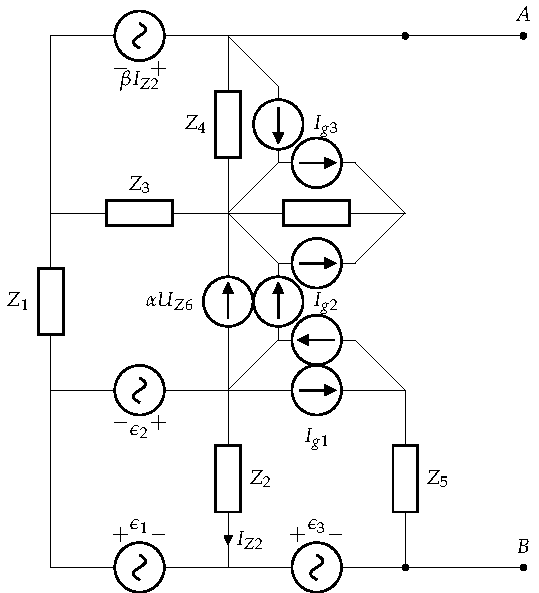
\includegraphics[scale=0.8]{figs/thevenin_movilidad.pdf}

  Esta transformación permite eliminar la rama de $Z_6$, dado que
  queda aislada. También permite cancelar las fuentes $I_{g1}$ e
  $I_{g2}$. Finalmente, $Z_5$ también queda aislada y puede eliminarse.

  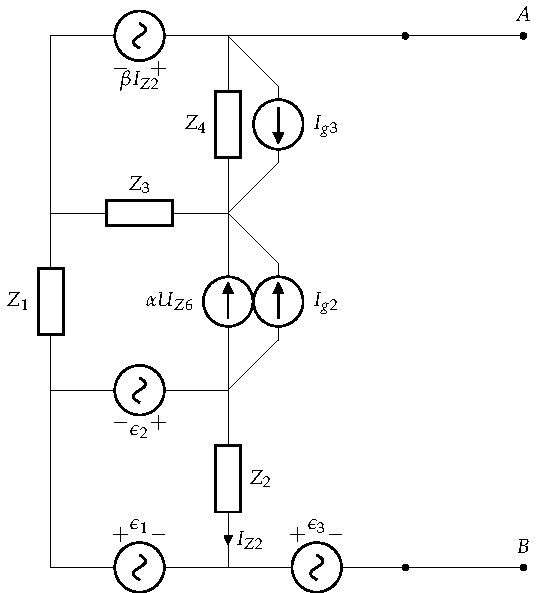
\includegraphics[scale=0.8]{figs/thevenin_movilidad2.pdf}

  A continuación, movemos la fuente $I_{g2}$ y la fuente dependiente.

  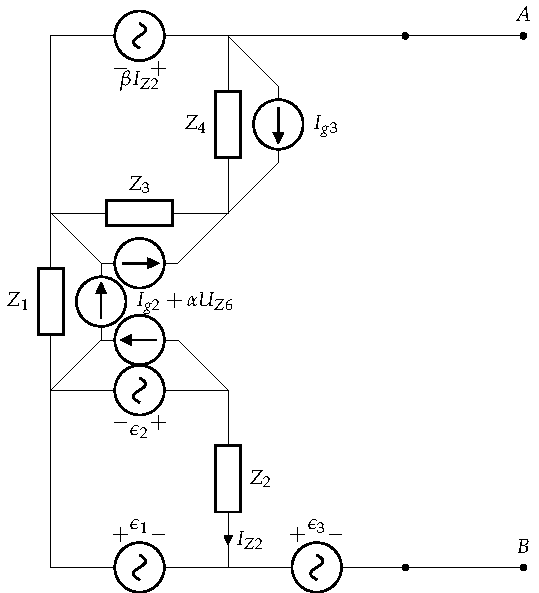
\includegraphics[scale=0.7]{figs/thevenin_movilidad3.pdf}

\item La fuente $\epsilon_2$ es dominante sobre las fuentes de
  corriente.

  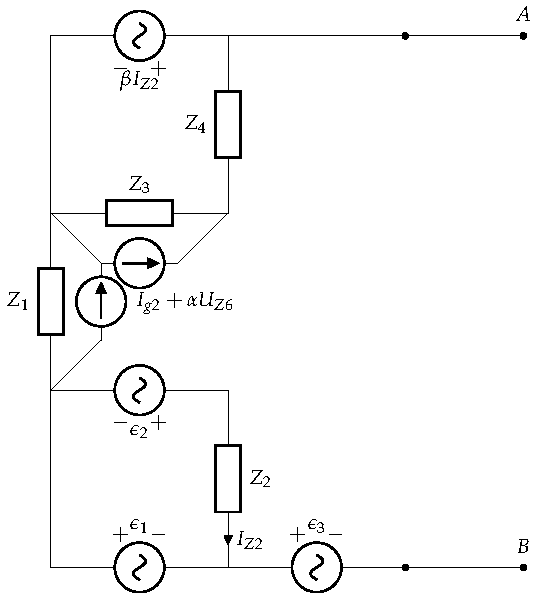
\includegraphics[scale=0.7]{figs/thevenin_dominancia.pdf}

  En este circuito, la fuente $\epsilon_1$ es dominante sobre la
  asociación de $\epsilon_2$ y $Z_2$. Asimismo, la fuente dependiente
  de tensión es dominante sobre la asociación de $Z_3$ (y la fuente de
  corriente) y $Z_4$.
  
    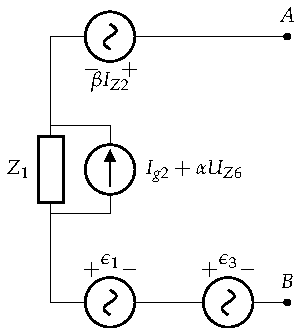
\includegraphics[]{figs/thevenin_dominancia2.pdf}
  
\item El circuito resultante permite calcular el generador equivalente
  de Thévenin:


  \begin{align*}
    \overline{\epsilon}_{th} &= \beta \overline{I}_{Z2} + \overline{Z}_1 (\overline{I}_{g2} + \alpha \overline{U}_{Z6}) + \overline{\epsilon}_1 + \overline{\epsilon}_3 = \SI[parse-numbers=false]{35 + 160 j}{\volt}\\
    \overline{Z}_{th} &= \overline{Z}_1 = \SI{2}{\ohm}
  \end{align*}

  Por tanto, entre A y B se debe conectar una impedancia de
  $\SI{2}{\ohm}$.
   

\end{enumerate}
\clearpage

\section*{Acoplamientos}


En el circuito de la figura:
\begin{enumerate}
\item \textbf{(5p.)} Escribe las ecuaciones de mallas sin realizar la sustitución numérica.
\item \textbf{(2,5p.)} Tras realizar la sustitución numérica, resuelve las ecuaciones anteriores, y obtén las corrientes de rama indicadas.
\item \textbf{(2,5p.)} Realiza un balance de potencias activas.
\end{enumerate}

\begin{center}
  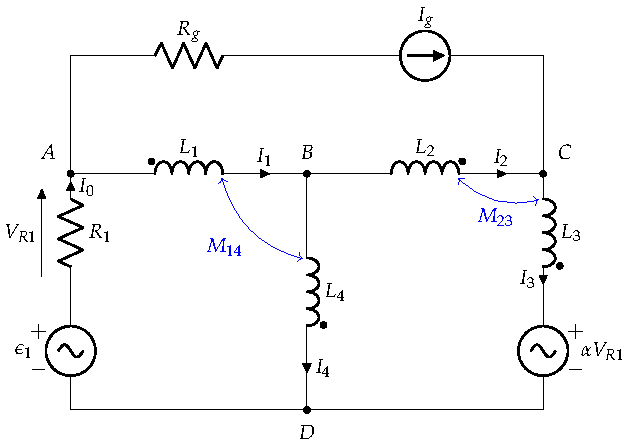
\includegraphics[height=0.4\textheight]{figs/acoplamientos_extra.pdf}
\end{center}

Datos:

\begin{align*}
  \overline{I}_g &= \SI[parse-numbers=false]{10\phase{\ang{0}}}{\ampere}\\
  \overline{\epsilon}_1 &= \SI[parse-numbers=false]{10\phase{\ang{0}}}{\ampere}\\
  R_i &= \SI{10}{\ohm} \quad \forall i\\
  X_{Li} &= \SI{10}{\ohm} \quad \forall i\\
  \alpha &= 2\\
\end{align*}

Todos los acoplamientos magnéticos del circuito son perfectos.
\subsection*{Solución}
Tomando las tres corrientes de malla en sentido dextrógiro, siendo $I_a$ la corriente de la malla inferior izquierda, $I_b$ la corriente de la malla inferior derecha, e $I_c$ la corriente de la malla superior, las ecuaciones de las dos mallas inferiores son:
\begin{align*}
  \overline{\epsilon}_1 &= \overline{I}_a (R_1 + j \omega L_1 + j \omega L_4 - 2 j \omega M_{14}) + \\
                        &+ \overline{I}_b (-j \omega L_4 + j \omega M_{14}) +\\
                        &+ \overline{I}_c (-j \omega L_1 + j \omega M_{14})
\end{align*}

\begin{align*}
  - \alpha \overline{U}_{R1} &= \overline{I}_a (- j \omega L_4 + j \omega M_{14}) + \\
                        &+ \overline{I}_b (j \omega L_4 + j\omega L_2 + j\omega L_3 + 2j\omega M_{23}) +\\
                        &+ \overline{I}_c (-j \omega L_2 - j \omega M_{23} - j\omega M_{14})
\end{align*}

Además,

\begin{align*}
  \overline{I}_c &= \overline{I}_g\\
  \overline{U}_{R1} &= R_1 \overline{I}_a
\end{align*}

Reagrupando obtenemos:
\begin{align*}
  \overline{\epsilon}_1 + \overline{I}_g (j \omega L_1 - j \omega M_{14}) &= \overline{I}_a (R_1 + j \omega L_1 + j \omega L_4 - 2 j \omega M_{14}) +  \overline{I}_b (-j \omega L_4 + j \omega M_{14})\\
  \overline{I}_g (j \omega L_2 + j \omega M_{23} + j\omega M_o{14}) &= \overline{I}_a (\alpha R_1 - j \omega L_4 + j \omega M_{14}) + \overline{I}_b (j \omega L_4 + j\omega L_2 + j\omega L_3 + 2j\omega M_{23})
\end{align*}

Realizamos la sustitución numérica, 

\begin{align*}
  10 + 10 (j 10 - j 10) &= \overline{I}_a (10 + j 10 + j 10 - j 20) +  \overline{I}_b (-j 10 + j 10)\\
  10 (j 10 + j 10 + j10) &= \overline{I}_a (20 - j 10 + j10) + \overline{I}_b (j 10 + j 10 + j 10 + j 20)
\end{align*}
donde se ha tenido en cuenta que:

\begin{align*}
  \omega M_{14} &= \sqrt{\omega L_1 \cdot \omega L_4} = \SI{10}{\ohm}\\
  \omega M_{23} &= \sqrt{\omega L_2 \cdot \omega L_3} = \SI{10}{\ohm}
\end{align*}

Simplificamos:

\begin{align*}
  10 &= 10 \overline{I}_a\\
  300j &= \overline{I}_a (20) + \overline{I}_b (j 50)
\end{align*}

La solución de este sistema es:

\begin{align*}
  \overline{I}_a &= \SI[parse-numbers=false]{1\phase{\ang{0}}}{\ampere}\\
  \overline{I}_b &= \SI[parse-numbers=false]{6.01\phase{\ang{3.81}}}{\ampere} = \SI[parse-numbers=false]{6 + 0.4j}{\ampere}
\end{align*}

Las corrientes de rama indicadas son:

\begin{align*}
  \overline{I}_0 &= \SI[parse-numbers=false]{1\phase{0}}{\ampere}\\
  \overline{I}_1 &= \SI[parse-numbers=false]{9\phase{\pi}}{\ampere}\\
  \overline{I}_2 &= \SI[parse-numbers=false]{-4 + 0.4j}{\ampere}\\
  \overline{I}_3 &= \SI[parse-numbers=false]{6 + 0.4j}{\ampere}\\
  \overline{I}_4 &= \SI[parse-numbers=false]{-5 - 0.4j}{\ampere}
\end{align*}

Finalmente, las potencias activas de los generadores son:

\begin{align*}
  P_{\epsilon1} &= Re(\overline{\epsilon}_1 \cdot \overline{I}_0^*) = \SI{10}{\watt}\\
  P_{\alpha} &= Re(\alpha R_1 \overline{I}_0 \cdot (-\overline{I}_3)^*) = \SI{-120}{\watt}\\
  P_{Ig} &= Re(\overline{U}_{Ig} \cdot \overline{I}_g^*) = \SI{1120}{\watt}
\end{align*}
y por tanto, la potencia total de los generadores es $\SI{1010}{\watt}$. La tensión $U_{Ig}$ se calcula con:

\begin{align*}
  \overline{U}_{AC} &= \overline{U}_{Rg} - \overline{U}_{Ig}\\
  \overline{U}_{AC} &= - R_1 \overline{I}_0 + \overline{\epsilon}_1 - \alpha \overline{I}_0 R_1 - j \omega L_3 \overline{I}_3 - j \omega M_{23} \overline{I}_2\\
  \overline{U_{Ig}} &= \SI[parse-numbers=false]{112 + 20j}{\volt}
\end{align*}
  
Las potencias de las resistencias son:

\begin{align*}
  P_{R1} &= R_1 I_0^2 = \SI{10}{\watt}\\ 
  P_{Rg} &= R_g I_g^2 = \SI{1000}{\watt}
\end{align*}

Comprobamos que la potencia activa total entregada por las fuentes coincide con la potencia activa total consumida en las resistencias.

\end{document}

% Local Variables:
% ispell-local-dictionary: "castellano"
% End:

